\section{Introduction}
Blockchain technology has revolutionized the way we create trustless and decentralized applications, offering immense composability and the ability to build complex primitives. However, the blockchain landscape is far from homogeneous, with multiple ecosystems that are based on their own consensus protocols and offer varying security and operation features. 

Axelar\footnote{\url{https://axelar.network}} enables interoperability between diverse blockchain ecosystems. Axelar is a Cosmos\footnote{\url{https://cosmos.network}} blockchain, which aims to link the Cosmos ecosystem to non-Cosmos chains, such as Ethereum, Bitcoin, Polygon, and others.

Ethereum, in particular, is one of the most widely used blockchains, hosting a multitude of decentralized applications spanning various sectors, including finance, gaming, and governance\cite{wood,buterin}. Therefore, establishing a seamless and secure connection to Ethereum is of paramount importance for Axelar. This proposal focuses on building a trustless connection between Axelar and Ethereum.

\subsection{Current Construction}
Currently, Axelar relies on a Tendermint-based delegated proof-of-stake consensus mechanism~\cite{axelar-whitepaper,buchman2019latest}. In particular, validators lock stake in the Axelar chain and receive stake delegations from Axelar users. The top $70$ validators, based on the aggregate (self and delegated) stake, are chosen to participate in Axelar's consensus mechanism.

Axelar adopts a modular architecture to connect with different chains. Each connector module consists of two essential components. The first component verifies source chain data (e.g., Ethereum) into Axelar. The second component generates threshold signatures, which can be verified on the source chain. In this report, we focus exclusively on the former, that is verification of source chain data that are bridged into Axelar.

Currently, connectors utilize an on-chain voting mechanism within Axelar to verify transactions that occur on the source chain. The validators who participate in a connector attestation are called \emph{attestors}. To determine the voting power of an attestor, Axelar employs quadratic voting. Briefly, the voting power of an attestor is the square root of their total stake. This mechanism aims to ensure a fair distribution of influence among attestors, based on their stake. Attestors are required to run a full node of the source chain and have access to the full node's RPC (Remote Procedure Call) interface. This enables them to verify the finalized transactions on the source chain, before voting to bridge them on Axelar.

To bridge data from the source chain to Axelar, a user interacts with an Axelar smart contract on the source chain. Subsequently, the user accesses the connector module on Axelar and initiates a voting poll, which is viewed by attestors. For each poll, an attestor decides whether to vote for or against. To make an informed decision, the attestor queries the source chain's full node RPC and checks if the
transaction under question has been finalized on the source chain. If a poll receives sufficient attestations, it is accepted, otherwise it is rejected.

This voting process forms the basis of verifying the source chain data into Axelar.
Nonetheless, for the connector construction to function securely, both the source chain and Axelar are assumed safe and live. In addition, the (quadratic) voting power distribution among the attestors is assumed to have an honest majority.

\subsection{Problem Statement}
The current construction of Axelar relies on attestors running the full node of the source chain to verify transactions and vote in an informed manner. However, this imposes significant costs.\footnote{Indicatively, running a full Ethereum node requires $4+$ CPU cores, $16+$ GB RAM, at least $1$ TB SSD, and $25$ Mbps of stable connection (source: \url{https://www.quicknode.com/guides/infrastructure/node-setup/ethereum-full-node-vs-archive-node}).}
Furthermore, as the Axelar network expands its support for additional chains, attestors will be required to run an increasing number of full nodes to verify transactions from these source chains.

% This scalability bottleneck hampers the growth and efficiency of the Axelar network. 
In practice, attestors often rely on third-party service providers to run and maintain the full nodes on their behalf. 
% Unfortunately, the Axelar network lacks a mechanism to detect whether attestors are utilizing third-party providers or running the full nodes themselves --- in fact, it is unclear if such behavior is detectable.
% 
This poses a significant centralization risk within the Axelar network. With a few dominant third-party providers in the market, attestors are likely to use the same service provider.\footnote{For example, at times, $50$\% of Ethereum's transactions ran through one provider, Infura~\cite{infura}.} If the third-party provider experiences a temporary compromise or breach, the entire Axelar network becomes vulnerable to attacks. 

% In addition, collusion among attestors can also jeopardize Axelar's security. 

% In both situations outlined above, an honest Axelar validator who is not actively monitoring the source chain has no means to detect the attack and would accept incorrect data.

To address this challenge, we propose a construction that enables users and attestors to verify the consensus of the source chain within the Axelar execution layer. This is accomplished through light and super-light client constructions of the source chain. In this report, we explore several constructions for light and super-light clients tailored specifically for Ethereum. We then propose a construction that best aligns with the requirements of Axelar, aiming to mitigate centralization risks, enhance security, and improve scalability. Our construction makes use of Ethereum's sync committee and guarantees bridge safety, assuming at least one Axelar attestor is honest.

\begin{figure}
    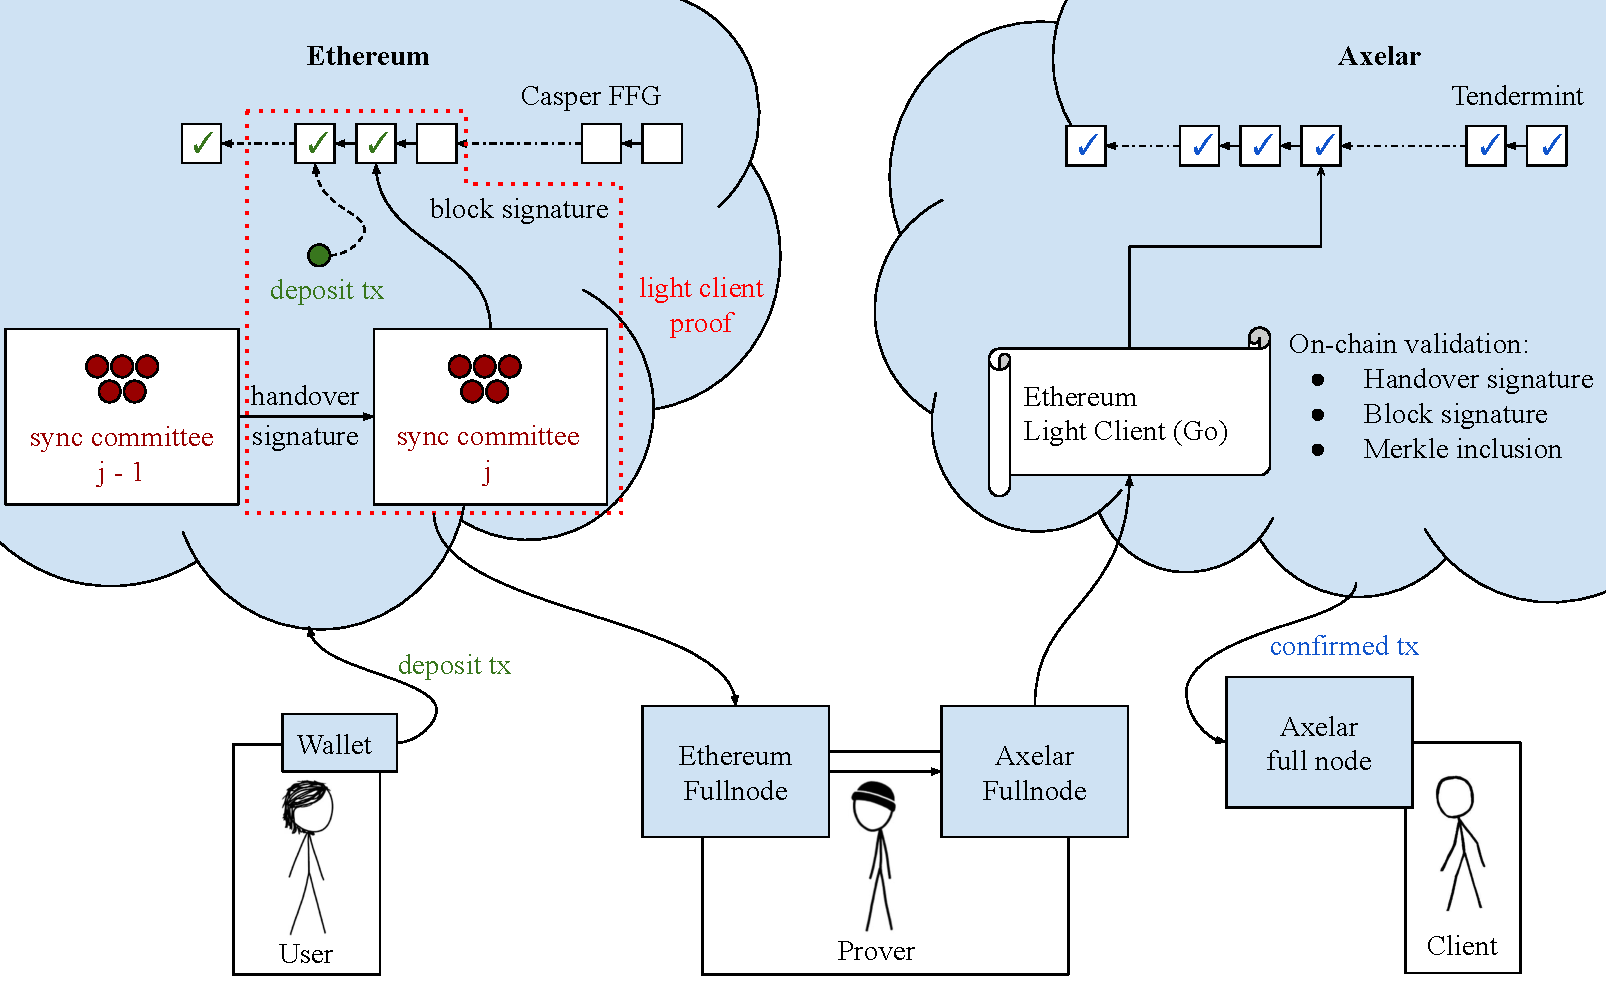
\includegraphics[scale=0.55]{figures/axelar_light_client_architecture.pdf}
    \caption{We recommend implementing an on chain light client using sync committee. The light client will be implemented as a go module that will be deployed on the Axelar network. The light client will be responsible for verifying the handover signatures, block signatures and Merkle inclusion proofs.}
    \label{fig.axelar_light_client_architecture}
\end{figure}


